% 渐屈线和渐伸线
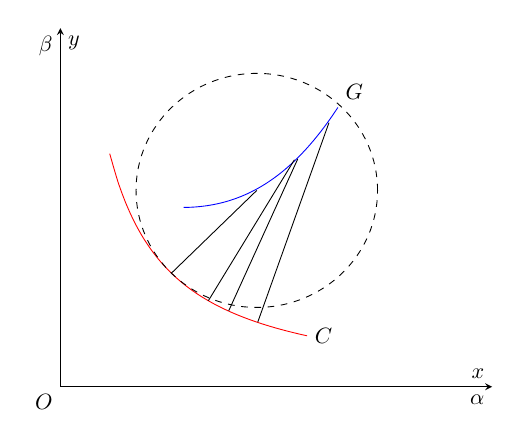
\begin{tikzpicture}[scale=0.8]
  \begin{axis}[clip=false,xmin=0, xmax=7,ymin=0,ymax=6, grid=none,
    xtick=\empty, ytick=\empty, axis lines=middle,
    smooth, xlabel={$x$}, ylabel={$y$}]

    \node [below left] at (0,6) {$\beta$};
    \node [below left] at (7,0) {$\alpha$};

    % 曲线 C
    % y' = -4/(x+0.2)^2
    % y'' = 8/(x+0.2)^3
    \node [right] at (4,0.85) {$C$};
    \addplot[draw=red,domain=0.8:4] {4/(x+0.2)-0.1};

    \node [above right] at (4.5,4.67) {$G$};
    \addplot[draw=blue,domain=2:4.5] {(x-2)^1.8/14*x + 3};

    \draw [dashed] (3.185,3.285) circle [radius=1.958];

    % (1.8,1.9)
    \addplot[domain=1.8:3.185] {x + 0.1};

    % (2.4,1.44)
    \addplot[domain=2.4:3.795] {1.69 * (x - 2.4) + 1.44};

    % (2.8,1.43)
    \addplot[domain=2.73:3.85] {2.27 * (x - 2.8) + 1.43};

    % (3.2,1.08)
    \addplot[domain=3.2:4.355] {2.89 * (x - 3.2) + 1.08};

    % 原点
    \node [below left] at (0,0) {$O$};
  \end{axis}
\end{tikzpicture}
